\documentclass{article} % For LaTeX2e
\usepackage{iclr2026_conference,times}
\input{math_commands.tex}

\usepackage{hyperref}
\usepackage{url}
\usepackage{graphicx}
\usepackage{booktabs}
\usepackage{multirow}
\usepackage{tabularx}
\usepackage{amsthm}
\usepackage{amsmath,amssymb}

\newtheorem{proposition}{Proposition}
\newtheorem{theorem}{Theorem}
\newtheorem{lemma}{Lemma}
\newtheorem{corollary}{Corollary}
\theoremstyle{remark}
\newtheorem{remark}{Remark}
\lhead{Under review as a conference paper at ICLR 2026}

\title{Last-Margin Gating Under a True Temporal Endpoint Data-Quality Shock}

\author{Anonymous}

\begin{document}

\maketitle

\begin{abstract}
Checkpoint policies are often evaluated under a fixed training distribution. We instead impose a
controlled temporal endpoint shock in synthetic sequence classification: labels remain clean until
a predetermined subset is flipped during the final quarter of training. A last-margin alarm compares
the final calibration loss with its running minimum, applies a threshold frozen on separate FIT
seeds, and rolls deployment back from \texttt{last} to best validation. On disjoint hold-out seeds,
the alarm detects all $64/64$ shocked runs and flags none of the $64$ healthy runs; rollback reduces
mean outer loss by $0.3395$ relative to \texttt{last}. However, every shocked trajectory reaches its
minimum immediately before the shock, so the gate, best-val, and early-stop return identical
outcomes. The experiment therefore supports contamination detection and rollback relative to
endpoint deployment, not discovery of a checkpoint unavailable to best-val. Healthy
$m\equiv0$ follows from strictly decreasing trajectories, leaving realistic deployment false alarms
unmeasured.
\end{abstract}

\section{Introduction}
\label{sec:intro}

A late event can invalidate an otherwise usable endpoint checkpoint. Static corruption does not
isolate this failure: when corruption is active from the first epoch, a poor final checkpoint does
not show that a previously clean candidate was later damaged. We construct the temporal case
directly, ending a clean prefix immediately before a final-quarter label shock. In every shocked
hold-out run, the checkpoint selected by best validation is recorded just before the shock begins
(Figure~\ref{fig:mechanism}).

We audit a simple deployment signal, the \emph{last margin}
$m=L_{11}-\min_{0\leq t\leq11}L_t$, where $L_t$ is calibration loss after epoch $t$. The signal is
read only at the end of the run. If $m$ exceeds a threshold calibrated without hold-out access, the
gate raises a contamination flag and deploys the best-validation checkpoint rather than
\texttt{last}. Figure~\ref{fig:mechanism} shows actual healthy and shocked trajectories, not a
schematic.

The experiment is pre-registered and deliberately narrow. Separate FIT seeds calibrate the
threshold; disjoint hold-out seeds settle detection and checkpoint outcomes
(Tables~\ref{tab:config} and~\ref{tab:runs}). The endpoint default is damaged, whereas the gate rolls
each affected run back to the same pre-shock checkpoint selected by best-val and early-stop
(Tables~\ref{tab:arms} and~\ref{tab:pairs}). This distinction---measurable value versus
\texttt{last}, but no checkpoint advantage over existing selectors---sets the scope of the paper.

Our contributions are:
\begin{enumerate}
\item a timing-controlled endpoint-shock protocol with a frozen FIT/hold-out split;
\item a paired measurement of alarmed rollback versus \texttt{last}; and
\item an explicit boundary: the gate does not outperform best-val or early-stop here, and the
healthy carrier does not measure realistic false alarms.
\end{enumerate}

\section{Related work}
\label{sec:related}

Weight averaging and checkpoint ensembling provide alternatives to endpoint deployment. Stochastic
weight averaging broadens the solution region \citep{swa}; exponential moving averages are widely
used to stabilize targets and model states \citep{ema}; and model soups combine multiple
fine-tuned checkpoints without additional inference cost \citep{wortsditcher2022}. We include
SWA, EMA, and soup as registered baselines, but our question is different: can a scalar read from
the completed trajectory attest that the final endpoint was exposed to a late event?

Robustness work shows that nominal accuracy and robustness objectives can diverge
\citep{labelnoise}. We use that citation only to motivate corruption as a stress test; it is not
evidence about temporal label shocks, nor do we propose a label-noise correction method. Our
contribution is the timing-controlled audit and its detection-versus-selection interpretation.

\section{Method}
\label{sec:method}

\subsection{A true temporal endpoint shock}
\label{sec:setting}

A run produces one calibration loss $L_t$ and one model snapshot after each of $E=12$ epochs. The
shocked mode starts from the same clean training examples as the healthy mode. A predetermined
subset of 150 of the 600 training examples is designated as affected. Crucially, designation does
not change any label during epochs $0,\ldots,8$. The command-line control
\texttt{--shock-time-frac}$=0.25$ sets
\begin{equation}
 t_{\mathrm{shock}}=\left\lceil(1-0.25)E\right\rceil=9.
\end{equation}
During epochs $9,10,11$ only, the affected examples use the deterministic target map
$y\mapsto(y+1)\bmod K$; all other labels remain clean. Epoch shuffling changes batch order but not
this onset. The intervention is therefore a time-gated late-training event, rather than a claim
that sample identity encodes training time.

The observed timeline validates the intended mechanism. All 64 shocked trajectories attain their
minimum at epoch 8, immediately before $t_{\mathrm{shock}}=9$, and all subsequent shocked points
remain above that minimum. Thus the clean candidate that later becomes best-val exists before the
intervention, while \texttt{last} is recorded after three affected epochs.

\begin{figure*}[t]
\centering
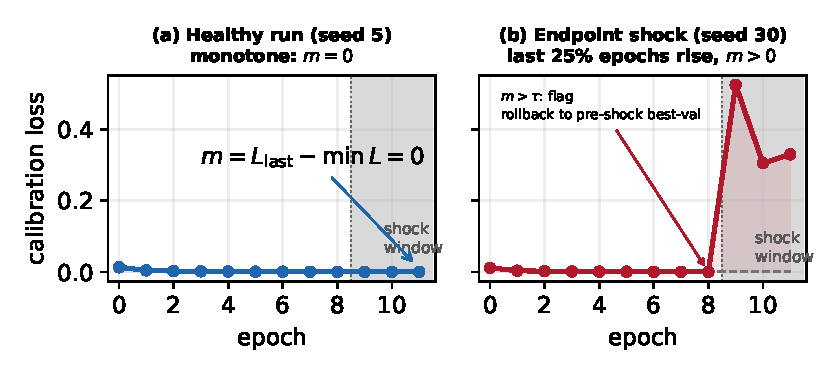
\includegraphics[width=0.88\textwidth]{figures/fig_mech_e1.pdf}
\caption{Actual E1 calibration trajectories. \textbf{Left:} healthy seed 5 decreases throughout,
so the final point is the minimum and $m=0$. \textbf{Right:} shocked seed 30 is clean through epoch
8; label flips activate only in the shaded epoch-9--11 window, lifting the trajectory above its
pre-shock minimum. The frozen-threshold gate flags the run and returns that pre-shock best-val
checkpoint. These representative runs were selected deterministically as closest to the
across-run median trajectory; aggregate results use all 64 seeds per arm.}
\label{fig:mechanism}
\end{figure*}

\subsection{Last-margin gate}
\label{sec:gate}

Define
\begin{equation}
 m=L_{E-1}-\min_{0\leq t<E}L_t\geq0.
\end{equation}
The gate is
\begin{equation}
\label{eq:gate}
\operatorname{gate}(m,\tau)=
\begin{cases}
\text{best-validation checkpoint}, & m>\tau,\\
\text{last checkpoint}, & m\leq\tau.
\end{cases}
\end{equation}
Firing is both an alarm and a rollback decision. The gate cannot return a checkpoint outside the
pair \{last, best-val\}; consequently, its scientific value must be stated relative to the endpoint
deployment it replaces, not as a new optimizer.

\subsection{Frozen calibration and comparison rules}
\label{sec:calibration}

Let $H$ and $S$ be the healthy and shocked last margins from four FIT seeds in each mode. Before
examining the hold-out settlement, we freeze
\begin{equation}
 \tau=\tfrac12\left(\max H+\min S\right)=0.1354038956.
\end{equation}
No hold-out trajectory is used to adjust this value. The registered comparison set contains the
endpoint, validation, stopping, averaging, soup, and rollback policies summarized with the full
configuration in Table~\ref{tab:config}.

\subsection{Settlement estimands}
\label{sec:settlement}

The primary alarm endpoints are recall on shocked runs and false-alarm rate (FAR) on healthy runs,
with one-sided 95\% Clopper--Pearson bounds. Checkpoint value is measured on the shocked arm by the
paired increment
\begin{equation}
 \Delta_{\mathrm{inc}}=
 \mathbb{E}\left[L_{\mathrm{outer}}(\mathrm{gate})-
 L_{\mathrm{outer}}(\mathrm{last})\right].
\end{equation}
The positive control reverses the endpoints,
$L_{\mathrm{outer}}(\mathrm{last})-L_{\mathrm{outer}}(\mathrm{best\text{-}val})$, to verify that
the late event actually damages endpoint deployment. We use the frozen paired bootstrap intervals
and one-sided sign-flip permutation results in the settlement artifact; exact selector identity is
reported as an equality rather than converted into a significance claim.

\section{Experimental setup}
\label{sec:exp}

\subsection{Carrier and run inventory}
\label{sec:configuration}

The carrier is a self-contained 5-class sequence-classification task trained on CPU. FIT and
hold-out seeds are disjoint, and training, calibration, and outer splits are disjoint within each
run. Table~\ref{tab:config} moves the complete configuration out of prose; Table~\ref{tab:runs} in
the appendix records every settlement unit.

\begin{table}[t]
\centering
\caption{Registered E1 configuration. The two fractions refer to different objects: 25\% of
examples are designated as affected, and their labels change only during the final 25\% of epochs.}
\label{tab:config}
\small
\begin{tabularx}{\linewidth}{@{}lX@{}}
\toprule
\textbf{Component} & \textbf{Setting} \\
\midrule
Task & 5 classes; vocabulary 400; sequence length 12; 6 informative features per class \\
Splits & train 600; calibration 200; outer 200; disjoint within each run \\
Model & 3-layer transformer; hidden size 64; 4 heads; feed-forward size 128 \\
Optimization & 12 epochs; batch 32; learning rate $3\times10^{-3}$; weight decay $0.01$ \\
Temporal shock & 150 affected examples; labels clean in epochs 0--8 and flipped in epochs 9--11 \\
Calibration & FIT seeds 101--104 in healthy and shocked modes; $\tau=0.1354$ \\
Settlement & hold-out seeds 1--64 in healthy and shocked modes \\
Selectors & last, best-val, early-stop, SWA, EMA, soup, rollback, margin-gate \\
\bottomrule
\end{tabularx}
\end{table}

\subsection{Pre-registration and frozen decision rule}
\label{sec:prereg}

The E1 pre-registration was frozen while only the first hold-out seed had completed. It declares
four pass conditions: the healthy FAR upper bound is at most $0.10$; at least one shocked run is
detected; the paired confidence interval for gate-minus-last is wholly below zero; and the paired
confidence interval for last-minus-best-val is wholly above zero. The settlement is a direct
execution of those conditions. We report all four, including the positive control that could have
invalidated the temporal-shock premise.

\section{Results}
\label{sec:results}

\subsection{The endpoint shock damages \texttt{last}, while pre-shock selectors survive}
\label{sec:rule-results}

Table~\ref{tab:arms} reports every registered checkpoint baseline on both modes and both outer
metrics. Under the endpoint shock, \texttt{last} has much higher loss than best-val and the gate;
its accuracy also falls while the pre-shock selectors remain perfect. Averaging baselines reduce
but do not eliminate the loss increase. The table retains every exact value and tied optimum.

\begin{table*}[t]
\centering
\caption{Mean outer outcomes over 64 hold-out seeds per mode. All rows are recomputed from the E1
raw run records. Bold marks the lowest shocked loss and highest shocked accuracy; equality is
retained rather than broken by arbitrary ranking.}
\label{tab:arms}
\small
\begin{tabular}{lcccc}
\toprule
& \multicolumn{2}{c}{\textbf{Healthy}} & \multicolumn{2}{c}{\textbf{Shocked}} \\
\cmidrule(lr){2-3}\cmidrule(lr){4-5}
\textbf{Rule} & \textbf{Outer loss} & \textbf{Outer accuracy} & \textbf{Outer loss} & \textbf{Outer accuracy} \\
\midrule
last        & 0.00063 & 1.00000 & 0.34046 & 0.95547 \\
best-val    & 0.00063 & 1.00000 & \textbf{0.00092} & \textbf{1.00000} \\
early-stop  & 0.00063 & 1.00000 & \textbf{0.00092} & \textbf{1.00000} \\
SWA         & 0.00088 & 1.00000 & 0.09780 & 0.99227 \\
EMA         & 0.00238 & 1.00000 & 0.03900 & 0.99531 \\
soup        & 0.00164 & 1.00000 & 0.02812 & 0.99680 \\
rollback    & 0.00070 & 1.00000 & 0.00106 & \textbf{1.00000} \\
margin-gate & 0.00063 & 1.00000 & \textbf{0.00092} & \textbf{1.00000} \\
\bottomrule
\end{tabular}
\end{table*}

The gate, best-val, and early-stop outcomes are exactly equal in all 64 shocked records, for both
outer loss and accuracy. Their common checkpoint is the epoch-8 snapshot. The alarm therefore
restores an existing pre-shock candidate rather than creating a better checkpoint.

\subsection{Paired endpoint effect and rollback increment}
\label{sec:paired-results}

Table~\ref{tab:pairs} gives the two frozen paired contrasts. The positive control establishes the
damage: \texttt{last} is worse than best-val by $+0.3395$. Turning on the gate relative to accepting
\texttt{last} changes the same quantity with the opposite sign, $-0.3395$. Both intervals exclude
zero by a wide margin, and the one-sided permutation estimates are approximately zero. The
per-run positive controls are shown in Figure~\ref{fig:paired}.

\begin{table}[t]
\centering
\caption{Frozen E1 paired outer-loss settlement on the 64 shocked hold-out runs. The two
bootstrap intervals were computed separately, so their endpoints are reported exactly as stored.
Permutation $p\approx0$ means zero counter-direction draws in the recomputed one-sided sign-flip
settlement.}
\label{tab:pairs}
\small
\begin{tabular}{lccc}
\toprule
\textbf{Contrast} & \textbf{Mean} & \textbf{95\% CI} & \textbf{One-sided $p$} \\
\midrule
gate $-$ last & $-0.3395$ & $[-0.3643,-0.3189]$ & $\approx0$ \\
last $-$ best-val & $+0.3395$ & $[0.3187,0.3634]$ & $\approx0$ \\
gate $-$ best-val & $0$ & exact equality in $64/64$ & not applicable \\
gate $-$ early-stop & $0$ & exact equality in $64/64$ & not applicable \\
\bottomrule
\end{tabular}
\end{table}

\begin{figure}[t]
\centering
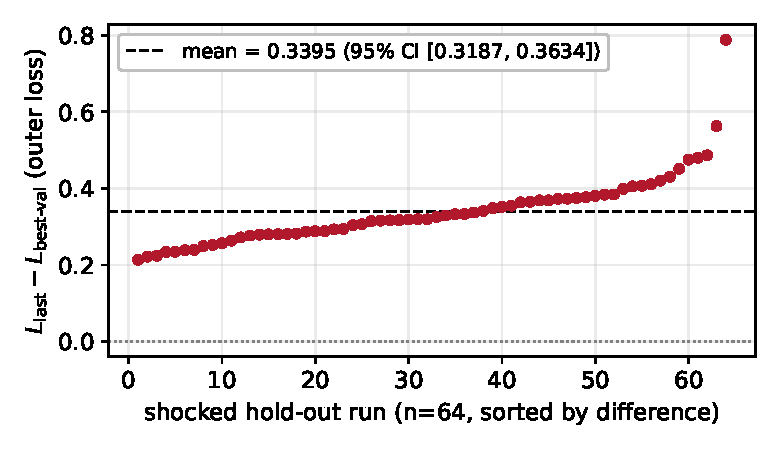
\includegraphics[width=0.88\linewidth]{figures/fig_paired_e1.pdf}
\caption{Per-run positive control
$L_{\mathrm{outer}}(\mathrm{last})-L_{\mathrm{outer}}(\mathrm{best\text{-}val})$ on 64 shocked
hold-out runs, sorted. The mean is $+0.3395$ and the 95\% CI is $[0.3187,0.3634]$, read directly
from the E1 settlement by the plotting script. Every observed difference is positive.}
\label{fig:paired}
\end{figure}

\subsection{Alarm operating characteristics}
\label{sec:operating}

At the FIT-frozen $\tau=0.1354$, every shocked margin exceeds the threshold and every healthy
margin equals zero. Table~\ref{tab:operating} reports both point estimates and the pre-registered
one-sided uncertainty bounds; Figure~\ref{fig:ecdf} shows the complete empirical distributions.

\begin{table}[t]
\centering
\caption{Alarm operating characteristics at frozen $\tau=0.1354$. Bounds are one-sided exact 95\%
Clopper--Pearson intervals in the conservative direction.}
\label{tab:operating}
\small
\begin{tabular}{lccc}
\toprule
\textbf{Endpoint} & \textbf{Count} & \textbf{Estimate} & \textbf{Exact bound} \\
\midrule
Recall on shocked runs & $64/64$ & $1.0$ & lower $0.9543$ \\
FAR on healthy runs & $0/64$ & $0.0$ & upper $0.0457$ \\
\bottomrule
\end{tabular}
\end{table}

\begin{figure}[t]
\centering
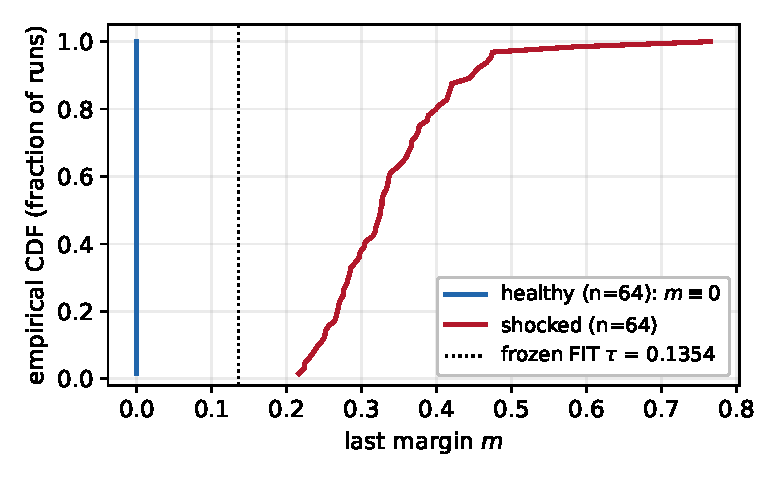
\includegraphics[width=0.88\linewidth]{figures/fig_margin_ecdf_e1.pdf}
\caption{Empirical CDF of the last margin over all E1 hold-out runs. Healthy margins are exactly
zero; shocked margins are dispersed but all exceed the FIT-frozen $\tau=0.1354$. The separation
supports the reported E1 operating point only; it is not a deployment calibration curve.}
\label{fig:ecdf}
\end{figure}

\subsection{The zero false-alarm rate is a design exclusion, not deployment evidence}
\label{sec:falsealarms}

FAR $=0$ is a real observation on this carrier, but the carrier excludes non-zero healthy margins.
Every healthy trajectory is strictly decreasing at every adjacent transition, so its final point
is necessarily the minimum and $m\equiv0$. Table~\ref{tab:healthy-audit} distinguishes this
mechanism from whole-cell readout collapse using the complete transition count and independent
outer-loss and accuracy readouts.

\begin{table}[t]
\centering
\caption{Independent audit of the healthy $m\equiv0$ cell. The observations distinguish a genuine
monotone signature from an all-zero or non-responsive readout.}
\label{tab:healthy-audit}
\small
\begin{tabular}{lcc}
\toprule
\textbf{Diagnostic} & \textbf{Observed} & \textbf{Interpretation} \\
\midrule
Strict adjacent decreases & $704/704$ & trajectory changes at every step \\
Argmin at final epoch & $64/64$ & monotone mechanism for $m=0$ \\
Best-val outer loss & mean $0.000625$ & non-zero independent loss readout \\
Best-val outer accuracy & $1.0$ in $64/64$ & task solved, not a dead cell \\
\bottomrule
\end{tabular}
\end{table}

The exact FAR bound therefore applies only to the registered monotone healthy population. A real
fine-tuning carrier with normal stochastic non-monotonicity is required to measure the deployment
false-alarm distribution; E1 does not supply that carrier.

\subsection{Interpretation and boundary of the result}
\label{sec:interpretation}

\subsubsection{The flag has measurable endpoint value, but does not discover a new checkpoint}
\label{sec:flag-value}

Relative to the experimental deployment default, the flag prevents deployment of the damaged final
snapshot, giving $\Delta_{\mathrm{inc}}=-0.3395$. Best-val and early-stop require no alarm to obtain
the same epoch-8 checkpoint. The supported claim is therefore \emph{detection plus rollback relative
to last}, not gate dominance over checkpoint selection.

The decisive next construction is E2: activate a shock early enough, or strongly enough, to
suppress or displace the clean argmin so that best-val itself fails. If gate and best-val remain
coextensive there, the checkpoint-novelty claim is falsified; if they separate under a frozen rule,
that experiment would test a contribution E1 cannot establish.

\section{Discussion}
\label{sec:discussion}

Because the affected labels activate only after a clean prefix, the experiment establishes the
ordering needed for an endpoint-shock audit: pre-shock minimum, shock onset, and damaged final
deployment. The paired benefit and positive control in Table~\ref{tab:pairs} quantify this same
operational event from opposite directions.

The meaningful policy comparison is correspondingly narrow. The gate has measured value against
\texttt{last}, but no checkpoint advantage over best-val or early-stop. SWA, EMA, soup, and rollback
also absorb much of the late shock (Table~\ref{tab:arms}), so the experiment does not establish that
an explicit alarm is necessary when a pipeline already deploys a pre-shock selector.

Table~\ref{tab:scope} makes the evidential boundary explicit. In particular, the healthy result is
internally valid but externally narrow: strict monotonicity is verified as a real signal, yet it
removes the variation needed for a realistic FAR test.

\begin{table}[h]
\centering
\caption{Claim boundaries and decisive next evidence. A checked E1 observation is not promoted
beyond the population or policy comparison that generated it.}
\label{tab:scope}
\small
\begin{tabularx}{\linewidth}{@{}lXX@{}}
\toprule
\textbf{Question} & \textbf{What E1 establishes} & \textbf{What remains open} \\
\midrule
Temporal integrity & Flips activate only in epochs 9--11 & Other shock types and durations \\
Alarm detection & Recall $1.0$ at frozen $\tau$ & Recall on a realistic carrier \\
Endpoint value & Gate beats \texttt{last} by $0.3395$ loss & Gate advantage over best-val (E2) \\
False alarms & FAR $0.0$ on verified monotone runs & FAR with natural non-monotonicity (E6) \\
Route-1 probe & Prior 36-run probe used a smaller, different carrier & No transport of its rates to E1 \\
\bottomrule
\end{tabularx}
\end{table}

\section{Limitations}
\label{sec:limits}

\begin{enumerate}
\item \textbf{Synthetic scale and intervention.} The carrier is a small CPU-trained classifier.
The intervention flips a predetermined affected subset only in the final three epochs. This is a
true late-training event, but it is not an external incident occurring after training has ended,
and its effect size must not be transported to large-model fine-tuning.
\item \textbf{Healthy variation is excluded.} Table~\ref{tab:healthy-audit} verifies that healthy
$m\equiv0$ is a genuine monotone signature rather than readout collapse. Nevertheless, the absence
of healthy non-monotonicity makes FAR $=0$ partly a design exclusion. E6 requires a realistic
carrier before any deployment-safety claim.
\item \textbf{Best-val is not defeated.} Every shocked argmin occurs before shock onset, as shown
in Figure~\ref{fig:mechanism}, and gate, best-val, and early-stop therefore agree exactly. E1
measures the value of a flag relative to \texttt{last}; E2 must cover or suppress the argmin to test
whether a gate can add checkpoint value beyond best-val.
\item \textbf{Threshold transport is untested.} The midpoint $\tau=0.1354$ is blind to hold-out but
calibrated on the same synthetic mechanism. No E1 threshold sweep is used to claim a safe band, and
the frozen value is not a recommended deployment threshold.
\item \textbf{Secondary diagnostics use distinct carriers.} Route 3 is an in-sample overtraining
diagnostic, and the prior Route-1 probe uses a downsized configuration. Neither supplies an E1 FAR
estimate or a substitute for a realistic healthy carrier.
\end{enumerate}

\section{Conclusion}
\label{sec:conclusion}

Under a controlled final-quarter label shock, the FIT-frozen last-margin alarm detects all shocked
runs and rolls the damaged endpoint back to a pre-shock checkpoint. Its outer-loss benefit is
measured relative to \texttt{last}; it offers no checkpoint advantage over best-val or early-stop,
which return the same outcomes. Realistic false-alarm behavior and any advantage beyond existing
selectors remain unmeasured.

\section*{Reproducibility}

The frozen pre-registration, FIT threshold, 128 raw hold-out records, settlement JSON, verdict,
and deterministic figure script are included in the anonymous workspace. Table~\ref{tab:runs}
enumerates the run budget. Quantitative figures are generated only from registered E1 records; the
conceptual image-generation candidate described in the supplementary disclosure is not used as
experimental evidence. AI assisted language editing; every claim and number was checked against
the registered artifacts.

% P5_MAIN_TEXT_END
\label{p5:main-text-end}
\bibliographystyle{iclr2026_conference}
\bibliography{references}

\newpage
\appendix

\section{Run inventory and provenance}
\label{app:inventory}

\begin{table}[h]
\centering
\caption{E1 run inventory. FIT runs only calibrate $\tau$; all point estimates and uncertainty
reported for E1 use the 128 hold-out runs.}
\label{tab:runs}
\small
\begin{tabular}{lrrr}
\toprule
\textbf{Phase} & \textbf{Seeds} & \textbf{Modes} & \textbf{Runs} \\
\midrule
FIT calibration & 4 & healthy, shocked & 8 \\
Hold-out settlement & 64 & healthy & 64 \\
Hold-out settlement & 64 & shocked & 64 \\
\midrule
\textbf{Total} & & & \textbf{136} (8 FIT + 128 hold-out) \\
\bottomrule
\end{tabular}
\end{table}

The temporal mechanism is implemented in \path{experiments/code/combined.py}; the frozen run and
settlement procedure is in \path{experiments/code/run_e1_temporal_shock.sh}; the pre-registration
is \path{experiments/prereg/PREREG_E1_TEMPORAL.md}; and the frozen numerical settlement is
\path{results/three_arm_temporal/E1_SETTLEMENT_frac0.25.json}. The representative and aggregate
figures are reproduced by \path{experiments/code/p5_e1_figs.py}.

\section{Distinct Route-3 diagnostic}
\label{app:route3}

This prior diagnostic tests a different failure mode and does not validate E1. On its 48 in-sample
runs, positive last margin and low outer accuracy identify the same set, and last-margin and final-
loss thresholds tie. The rates below are descriptive rather than deployment estimates.

\begin{table}[h]
\centering
\caption{Route-3 in-sample overtraining diagnostic, reported separately from E1.}
\label{tab:route3}
\small
\begin{tabular}{lcc}
\toprule
\textbf{Statistic} & \textbf{Recall} & \textbf{FAR} \\
\midrule
last margin & $1.0000$ & $0.0000$ \\
final loss level & $1.0000$ & $0.0000$ \\
first-rise early-stop & $0.8929$ & $0.1000$ \\
non-monotonicity indicator & $1.0000$ & $0.1500$ \\
\bottomrule
\end{tabular}
\end{table}

\begin{figure}[h]
\centering
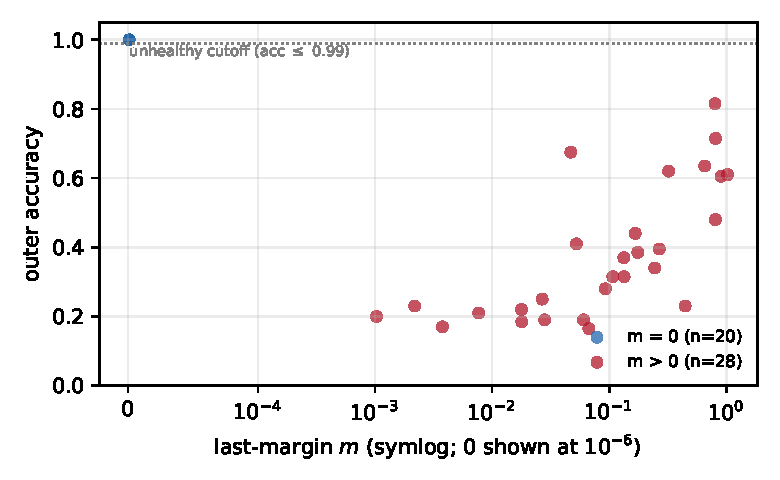
\includegraphics[width=0.78\linewidth]{figures/fig_route3.pdf}
\caption{Route-3 overtraining scatter, retained as a distinct diagnostic. On these 48 runs,
$m>0$ and outer accuracy $\leq0.99$ identify the same 28 runs. The identity explains the perfect
in-sample last-margin row in Table~\ref{tab:route3}; it does not provide an E1 operating estimate.}
\label{fig:route3}
\end{figure}

\section{Statistical details}
\label{app:statistics}

Recall and FAR bounds are one-sided 95\% Clopper--Pearson bounds. The two paired 95\% confidence
intervals in Table~\ref{tab:pairs} use the bootstrap distributions frozen in the E1 settlement.
The sign-flip permutation results were recomputed with 20,000 one-sided draws and correct
elementwise signs; the stored empirical values are zero, which we report as $p\approx0$ rather than
as mathematical probability zero. Exact equality statements for gate, best-val, and early-stop
come from recordwise equality of both stored outer loss and stored outer accuracy, not a null test.

\end{document}
